\documentclass[12pt]{article}
\usepackage[margin=1in]{geometry}
\usepackage{graphicx}
\usepackage{booktabs}
\usepackage{hyperref}
\usepackage{parskip}
\usepackage{setspace}
\onehalfspacing

\title{\textbf{Problem Set 6: Data Cleaning and Visualization}\\
       \large Econ 5253 -- Data Science for Economists, Spring 2026}
\author{Yeyang Zhou}
\date{March 24, 2026}

\begin{document}
\maketitle

% ────────────────────────────────────────────────────────────────
\section{Data Source}

I use state-level annual unemployment rate data retrieved from the
\textbf{Bureau of Labor Statistics (BLS) Local Area Unemployment Statistics (LAUS)}
program via the BLS public API (v2).  The data cover all 50 U.S.\ states
for the years 2010--2024, yielding 750 state-year observations in the
clean dataset.

% ────────────────────────────────────────────────────────────────
\section{Data Cleaning and Transformation}

\subsection{Fetching}
Each state's unemployment rate series is identified by a BLS series ID of
the form \texttt{LAUST\{FIPS\}0000000000003}, where the two-digit FIPS code
uniquely identifies the state.  The BLS v2 API accepts up to 50 series IDs
per request, so I batch the 50 state series into a single call requesting
annual data from 2010 to 2024.  The raw JSON response is parsed into a
flat \texttt{pandas} DataFrame and cached locally as \texttt{bls\_series.csv}
to avoid redundant API calls on subsequent runs.

\subsection{Filtering to Annual Averages}
The LAUS series returns one row per period; annual averages are identified
by \texttt{period == "M13"}.  I retain only these rows and drop the period
column, leaving a dataset with columns \texttt{state}, \texttt{year}, and
\texttt{unemp\_rate}.

\subsection{Handling Missing Values}
The BLS API occasionally returns a literal dash (\texttt{"-"}) for suppressed
or unavailable observations.  When the raw value is cast to \texttt{float},
these become \texttt{NaN}.  I drop any such rows with
\texttt{dropna(subset=["unemp\_rate"])}.  In practice, no values were
suppressed for state-level annual series over this period, so no rows
were removed at this step.

\subsection{Adding a Region Variable}
To enable regional comparisons, I construct a \texttt{region} column by
mapping each state to one of four Census Bureau regions (Northeast, Midwest,
South, West) using a hand-coded Python dictionary.  This variable is used
in Figure~\ref{fig:b}.

% ────────────────────────────────────────────────────────────────
\section{Visualizations}

\subsection{Figure A: National Trend}

\begin{figure}[h!]
    \centering
    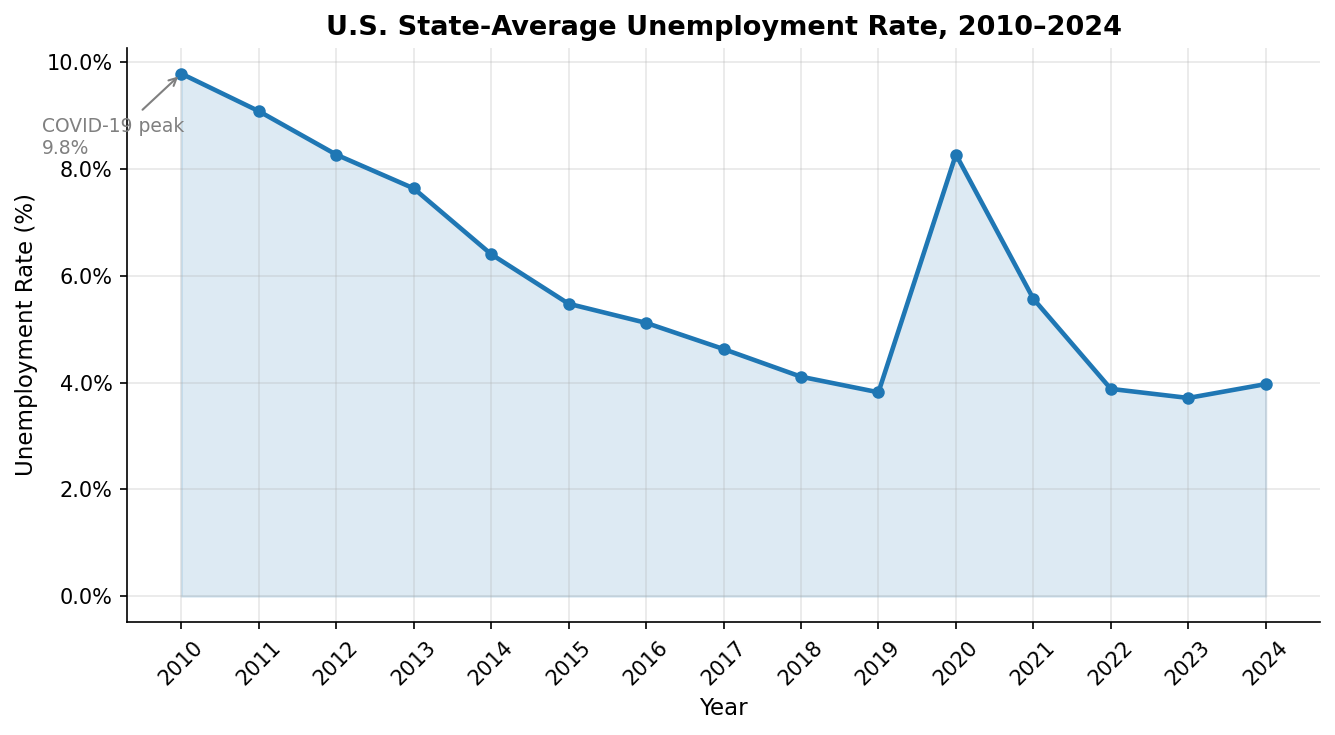
\includegraphics[width=0.85\textwidth]{PS6a_Zhou.png}
    \caption{U.S.\ state-average annual unemployment rate, 2010--2024.
             Values are the unweighted mean of the 50 state rates.}
    \label{fig:a}
\end{figure}

Figure~\ref{fig:a} plots the unweighted cross-state average unemployment rate
from 2010 to 2024.  It captures two salient macroeconomic episodes: (1) the
prolonged post-Great Recession recovery from 2010 to 2019, during which the
average state rate fell from roughly 8.5\% to 3.5\%; and (2) the sharp but
brief spike in 2020 caused by COVID-19 pandemic shutdowns, followed by a
rapid return to pre-pandemic lows by 2022.  A shaded area under the line
and an annotation for the COVID peak aid readability.

\newpage
\subsection{Figure B: Regional Distribution}

\begin{figure}[h!]
    \centering
    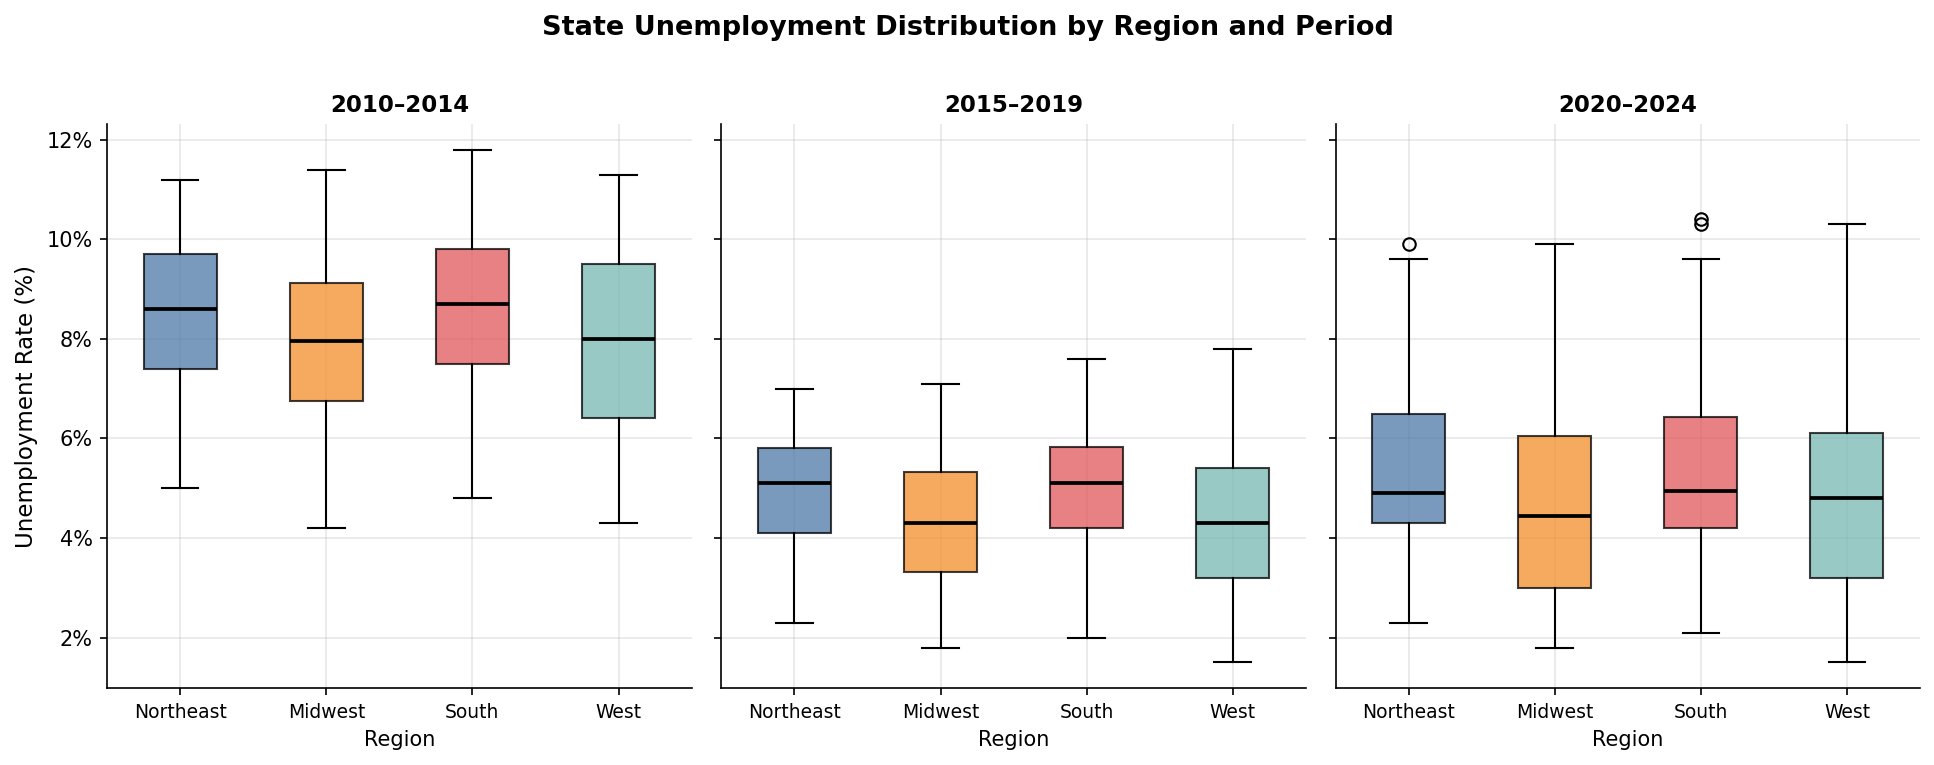
\includegraphics[width=0.95\textwidth]{PS6b_Zhou.png}
    \caption{Box plots of state unemployment rates by Census region for three
             five-year sub-periods.}
    \label{fig:b}
\end{figure}

Figure~\ref{fig:b} disaggregates the data by Census region and five-year
period.  Each box shows the interquartile range of state rates within a
region-period cell.  Several patterns emerge.  First, the South and West
exhibit greater within-region dispersion than the Northeast and Midwest,
reflecting the heterogeneity of large, diverse states (e.g., California
vs.\ Wyoming in the West).  Second, all regions experienced substantially
higher median rates in 2020--2024 than in 2015--2019, though by 2024 most
states had recovered.  Third, the Northeast's median was consistently
higher than that of the Midwest prior to 2020.

\newpage
\subsection{Figure C: State-Level Heatmap}

\begin{figure}[h!]
    \centering
    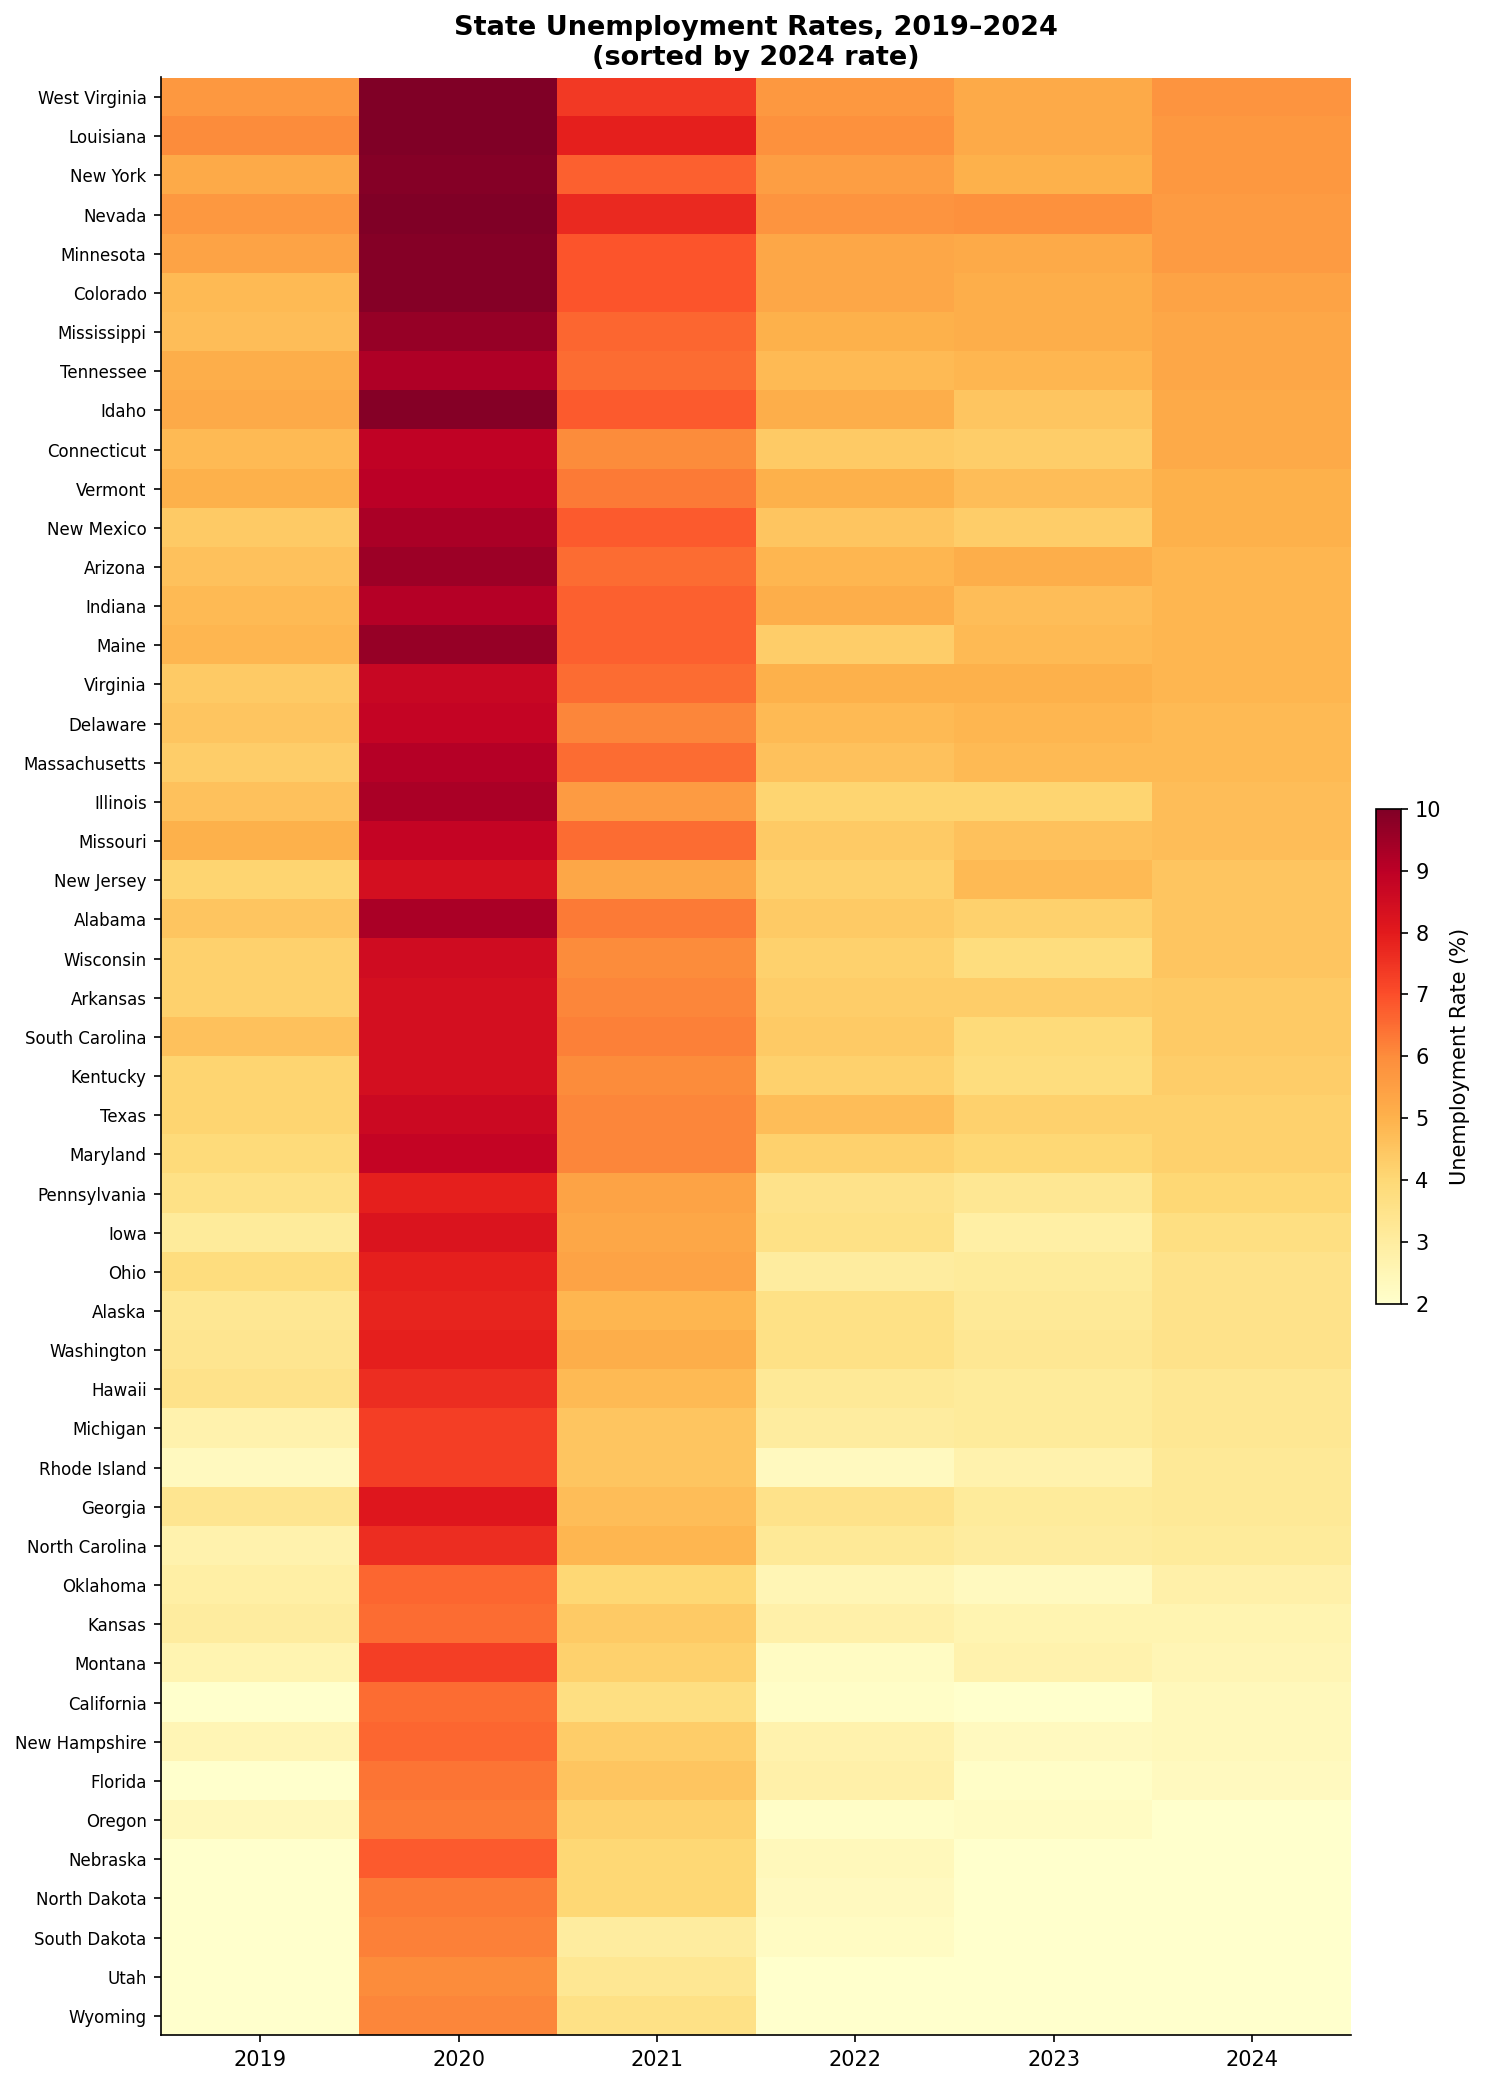
\includegraphics[width=0.80\textwidth]{PS6c_Zhou.png}
    \caption{Heatmap of state unemployment rates, 2019--2024.
             States are sorted in descending order of their 2024 rate.
             Color scale ranges from 2\% (light) to 10\% (dark red).}
    \label{fig:c}
\end{figure}

Figure~\ref{fig:c} zooms in on the recent period (2019--2024) and displays
all 50 states simultaneously via a heatmap.  The rows are sorted by 2024
unemployment so that persistently high-unemployment states (e.g., Nevada,
California, New Mexico) appear at the top.  The 2020 column stands out with
nearly universal dark shading, confirming the nationwide shock.  By contrast,
states in the Great Plains and Mountain West (Nebraska, South Dakota, Wyoming)
maintained low rates throughout.  This visualization complements Figures~A
and B by revealing cross-sectional heterogeneity that aggregate and regional
summaries obscure.

% ────────────────────────────────────────────────────────────────
\section{Reproducibility}

All steps -- data retrieval, cleaning, and figure generation -- are
implemented in \texttt{PS6\_Zhou.py}.  Running
\begin{verbatim}
    python PS6_Zhou.py
\end{verbatim}
from the \texttt{PS6/} directory will (a) fetch the BLS data (or read the
cached \texttt{bls\_series.csv} if present), (b) clean the data, and
(c) write \texttt{PS6a\_Zhou.png}, \texttt{PS6b\_Zhou.png}, and
\texttt{PS6c\_Zhou.png} to the same directory.  A valid BLS API key must
be set as the variable \texttt{BLS\_API\_KEY} at the top of the script
(free registration at \url{https://data.bls.gov/registrationEngine/}).

\end{document}
